% Reproduction Slides

\begin{frame}{Vision Results: Claims V1--V3}
    \begin{columns}[T]
        % V1: Low-rank emergence
        \column{0.3\textwidth}
        \fcolorbox{blue!50}{blue!5}{
            \parbox{0.95\textwidth}{
                \centering
                \textbf{V1: Low-rank emergence} \checkmark
                
                \vspace{0.05cm}
                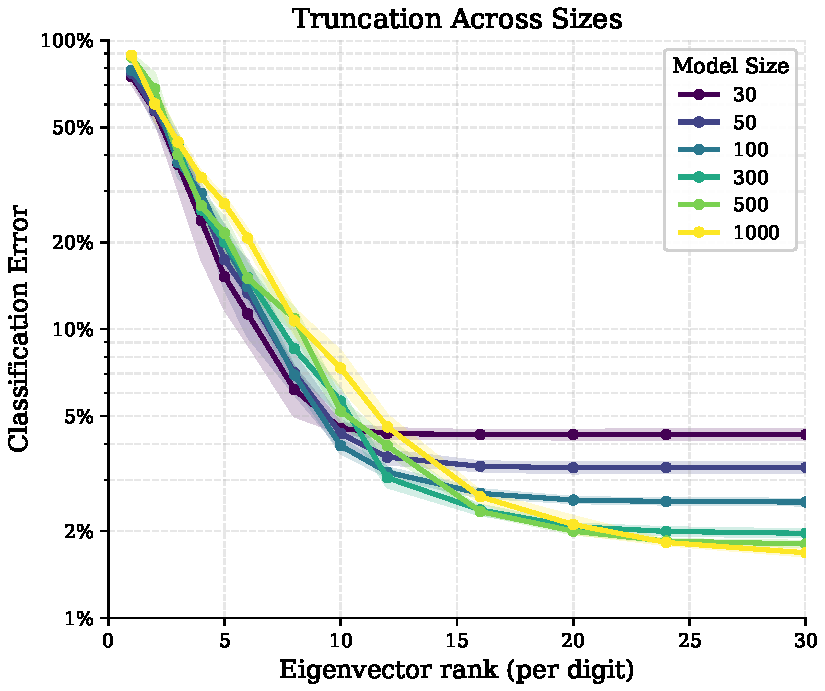
\includegraphics[width=0.95\textwidth,height=0.45\textheight,keepaspectratio]{../Report/figures/vision/figure_5b_truncation.pdf}
                
                \vspace{0.05cm}
                \scriptsize
                Top-$k$ truncation preserves accuracy
            }
        }
        
        % V2: Interpretable eigenvectors
        \column{0.35\textwidth}
        \fcolorbox{green!50}{green!5}{
            \parbox{0.95\textwidth}{
                \centering
                \textbf{V2: Interpretable eigenvectors} \checkmark
                
                \vspace{0.05cm}
                {\tiny Full Reg (noise+WD):}
                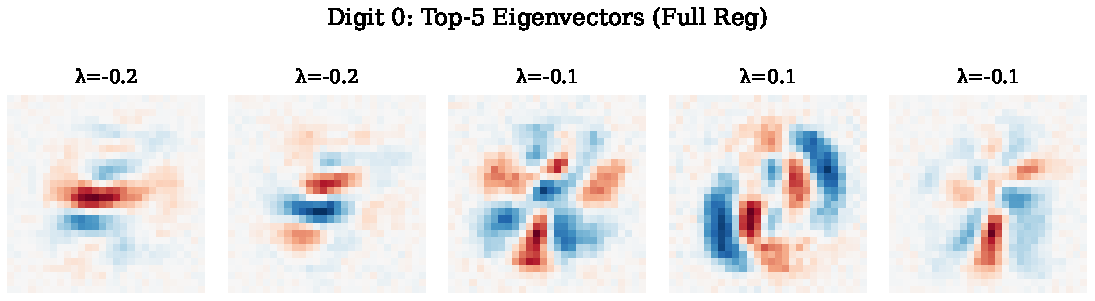
\includegraphics[width=0.95\textwidth,height=0.18\textheight,keepaspectratio]{../Report/figures/vision/eigenvectors_digit0_reg.pdf}
                
                \vspace{0.05cm}
                {\tiny Noise Only:}
                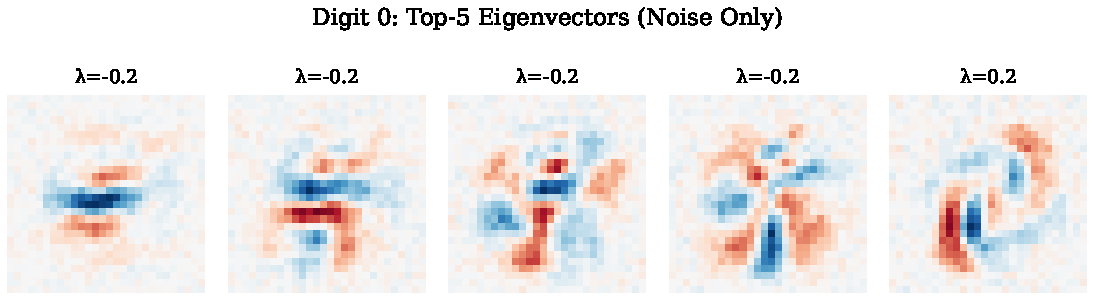
\includegraphics[width=0.95\textwidth,height=0.18\textheight,keepaspectratio]{../Report/figures/vision/eigenvectors_digit0_noise.pdf}
                
                \vspace{0.05cm}
                \scriptsize
                Both show clear ``0'' patterns
            }
        }
        
        % V3: Overfitting without reg
        \column{0.35\textwidth}
        \fcolorbox{red!50}{red!5}{
            \parbox{0.95\textwidth}{
                \centering
                \textbf{V3: Overfitting w/o reg} \checkmark
                
                \vspace{0.05cm}
                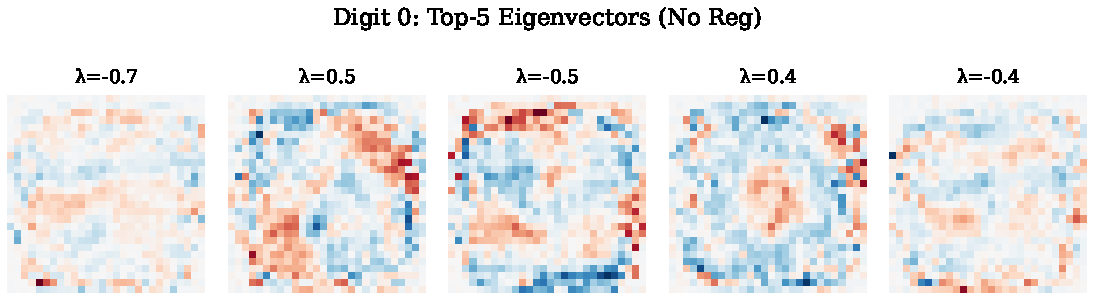
\includegraphics[width=0.95\textwidth,height=0.4\textheight,keepaspectratio]{../Report/figures/vision/eigenvectors_digit0_noreg.pdf}
                
                \vspace{0.05cm}
                \scriptsize
                Digit 0, no reg: diffuse, noisy
            }
        }
    \end{columns}
    
    \vspace{0.1cm}
    \centering
    \footnotesize
    \textbf{Key insight:} Regularization induces low-rank structure; \textbf{noise} makes eigenvectors interpretable.
\end{frame}

\begin{frame}{Vision Results: Claims V4--V6}
    \begin{columns}[T]
        % V4: Regularization roles
        \column{0.33\textwidth}
        \fcolorbox{blue!50}{blue!5}{
            \parbox{0.95\textwidth}{
                \centering
                \textbf{V4: Regularization roles} \checkmark
                
                \vspace{0.05cm}
                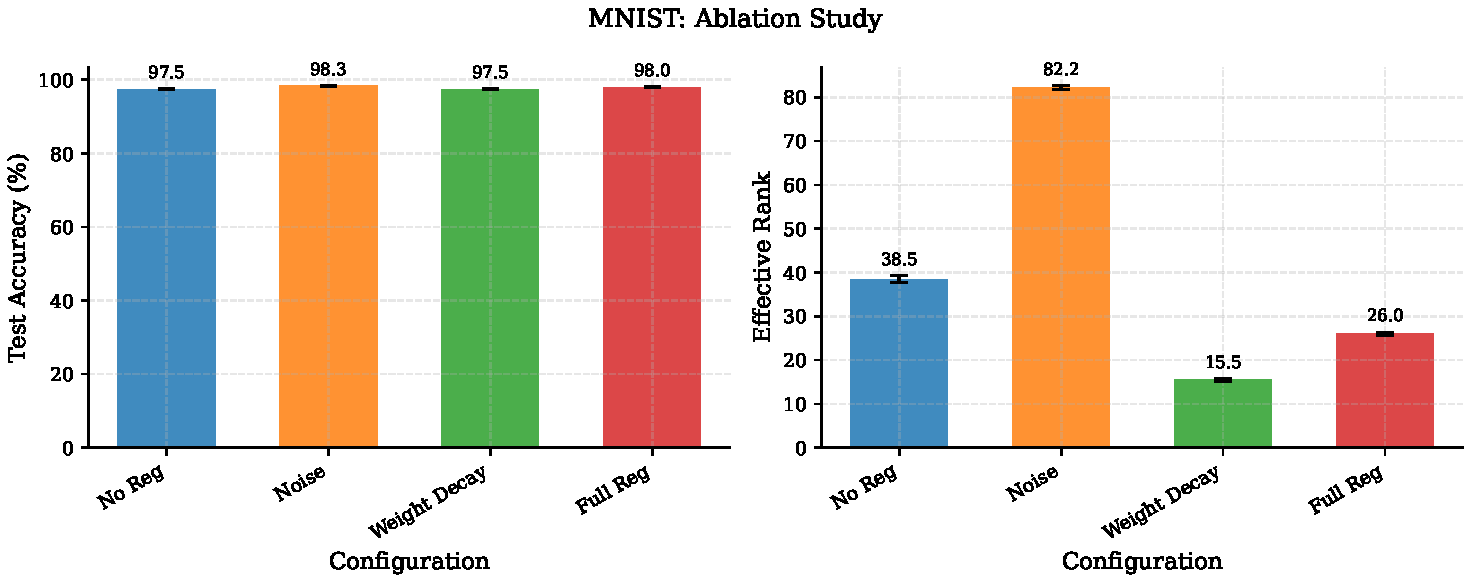
\includegraphics[width=0.95\textwidth,height=0.32\textheight,keepaspectratio]{../Report/figures/vision/mnist_ablation.pdf}
                
                \vspace{0.05cm}
                \scriptsize
                \textbf{WD} $\downarrow$ rank; \textbf{Noise} $\uparrow$ acc
                
                \vspace{0.05cm}
                \tiny
                EffRank ratio = $\frac{\text{EffRank(WD)}}{\text{EffRank(none)}}$\\
                $= \frac{15.5}{38.5} = 0.40 < 0.5$ \checkmark
            }
        }
        
        % V5: Cross-seed consistency
        \column{0.33\textwidth}
        \fcolorbox{green!50}{green!5}{
            \parbox{0.95\textwidth}{
                \centering
                \textbf{V5: Cross-seed consistency} \checkmark
                
                \vspace{0.05cm}
                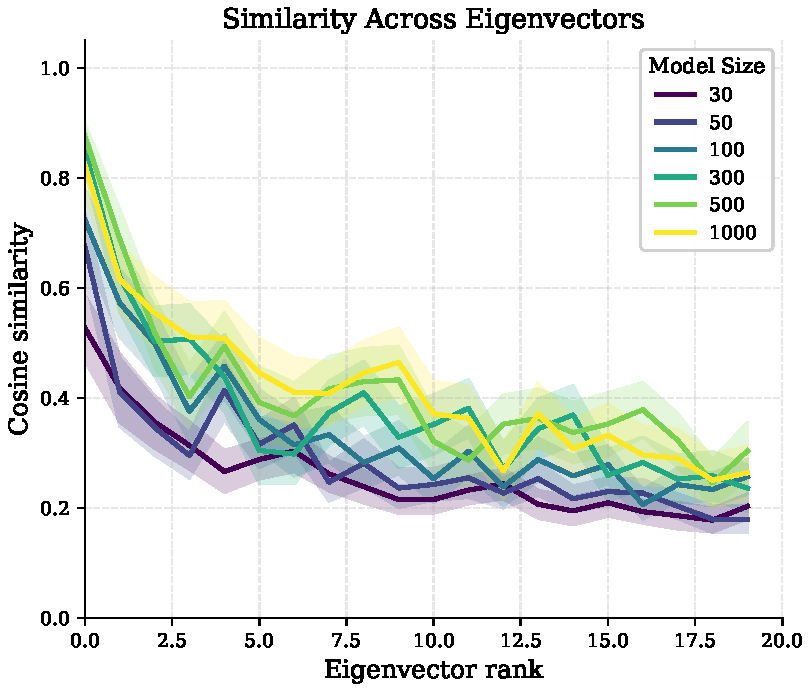
\includegraphics[width=0.95\textwidth,height=0.32\textheight,keepaspectratio]{../Report/figures/vision/figure_5a_similarity.pdf}
                
                \vspace{0.05cm}
                \scriptsize
                Top eigenvectors highly similar across seeds; similarity decays with rank
            }
        }
        
        % V6: Adversarial generation
        \column{0.33\textwidth}
        \fcolorbox{orange!50}{orange!5}{
            \parbox{0.95\textwidth}{
                \centering
                \textbf{V6: Adversarial gen.} \checkmark
                
                \vspace{0.05cm}
                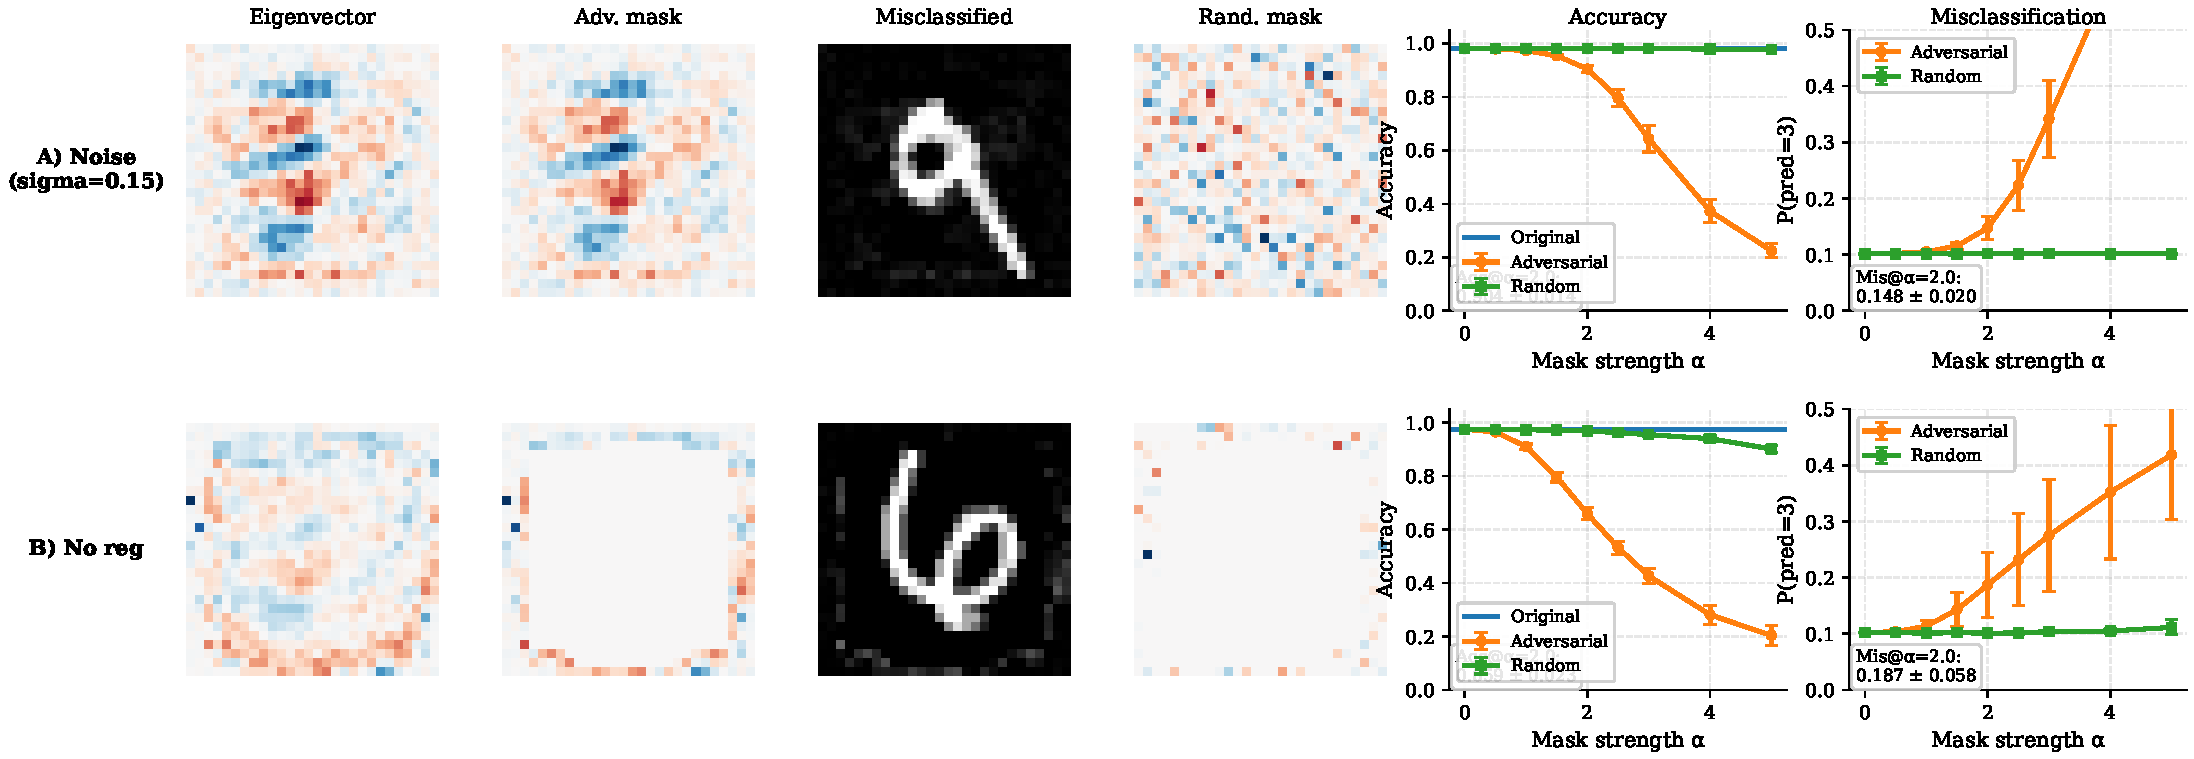
\includegraphics[width=0.95\textwidth,height=0.38\textheight,keepaspectratio]{../Report/figures/vision/figure_7_adversarial.pdf}
                
                \vspace{0.05cm}
                \scriptsize
                $\mathbf{m}_c = (V_c^+)^\dagger_{:,1}$: top positive eigenvector.\\
                Pseudoinverse extracts $V^+$ from $B_c$.\\
                \textbf{Result:} Eigenvector mask $>$ random.
            }
        }
    \end{columns}
    
    \vspace{0.1cm}
    \centering
    \footnotesize
    \textbf{All 6 vision claims reproduced.}
\end{frame}

\begin{frame}{Language Results: Claims L1, L2, L4 (Figure 8)}
    \begin{columns}[T]
        % LEFT: Methodology
        \column{0.32\textwidth}
        \small
        \textbf{Methodology:}
        
        \vspace{0.1cm}
        \scriptsize
        \textbf{1. Data:} Run $\sim$50k tokens, record MLP activations $\mathbf{h}^{\text{in}}, \mathbf{h}^{\text{out}}$.
        
        \vspace{0.05cm}
        \textbf{2. Encode:} Use pretrained SAEs:\\
        $\mathbf{z} = \text{TopK}(\mathbf{W}_{\text{enc}} \mathbf{h})$
        
        \vspace{0.05cm}
        \textbf{3. Build $Q_f$:} For output feature $f$:\\
        $z^{\text{out}}_f \approx (\mathbf{z}^{\text{in}})^\top Q_f \mathbf{z}^{\text{in}}$
        
        \vspace{0.05cm}
        \textbf{4. Analyze:} Eigendecompose $Q_f$, visualize structure.
        
        % RIGHT: Figure + Claims
        \column{0.68\textwidth}
        \centering
        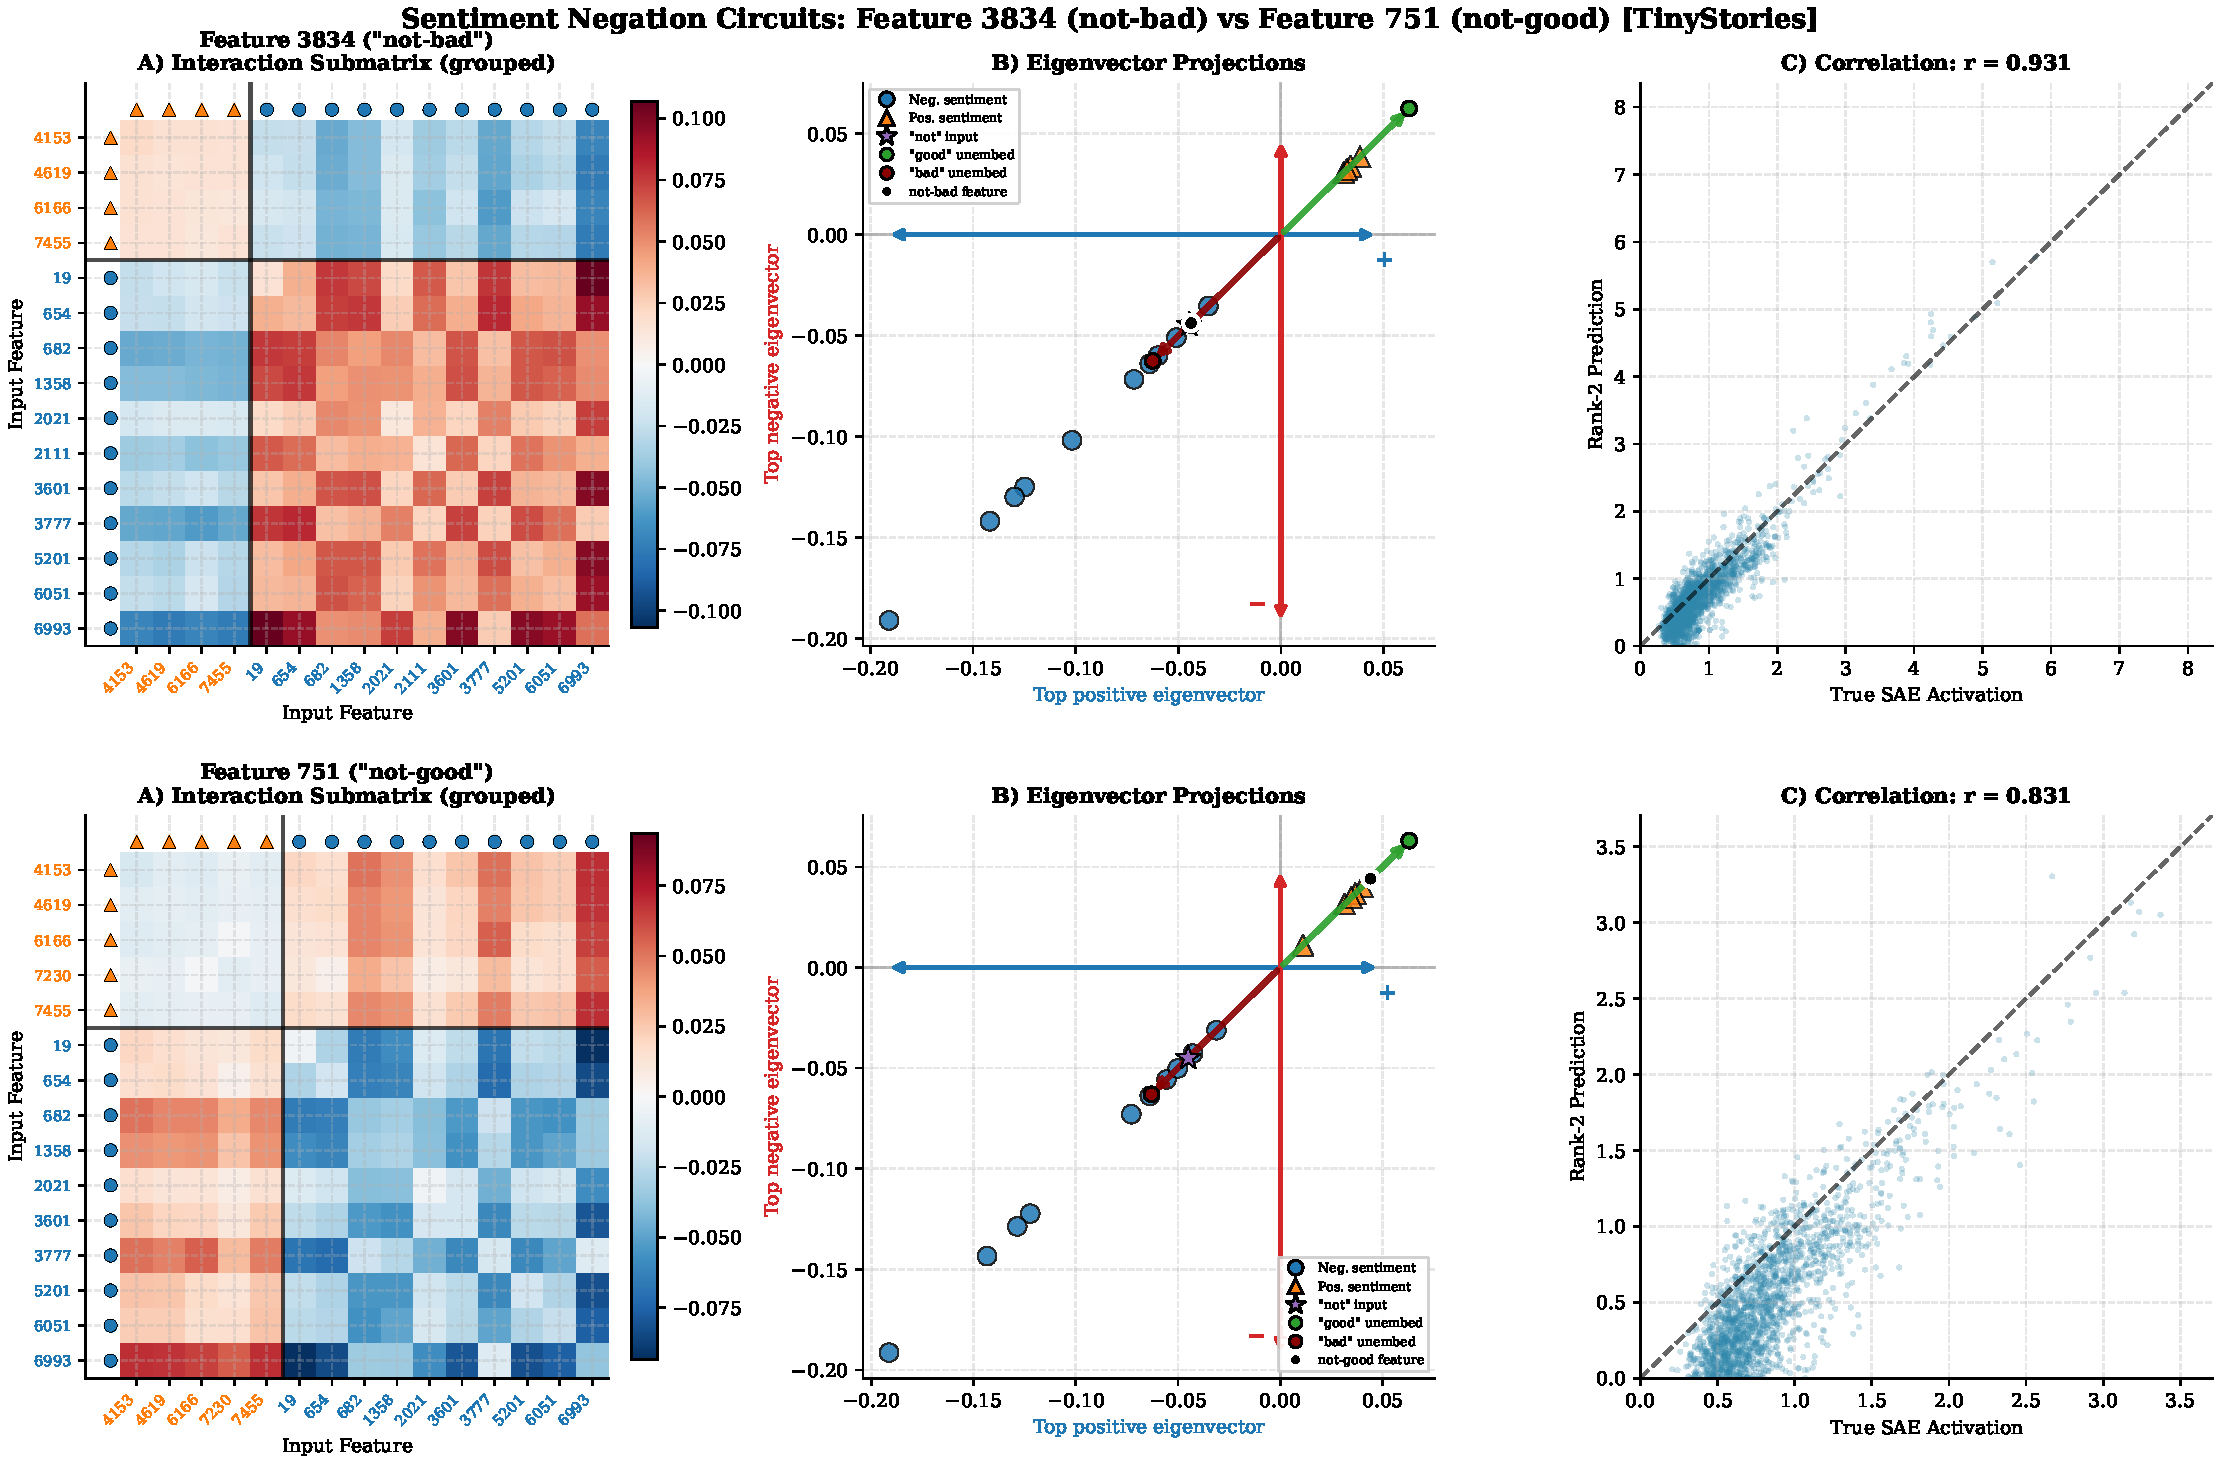
\includegraphics[width=\textwidth,height=0.38\textheight,keepaspectratio]{../Report/figures/language/figure_8_final.pdf}
        
    \end{columns}
    
    \vspace{0.1cm}
    \footnotesize
    \hspace{-0.3cm}
    \fcolorbox{blue!50}{blue!5}{
        \parbox{0.28\textwidth}{\scriptsize
            \textbf{L1: SAE discovery} \checkmark\\[0.05cm]
            SAEs find interpretable features (``not-good'', ``not-bad'')
        }
    }
    \hfill
    \fcolorbox{green!50}{green!5}{
        \parbox{0.28\textwidth}{\scriptsize
            \textbf{L2: Negation circuit} \checkmark\\[0.05cm]
            AND-gate confirmed: negation $\otimes$ sentiment
        }
    }
    \hfill
    \fcolorbox{orange!50}{orange!5}{
        \parbox{0.28\textwidth}{\scriptsize
            \textbf{L4: Sparse interact.} \checkmark\\[0.05cm]
            $Q_f$ shows clear block structure
        }
    }
    
    \vspace{0.1cm}
    \hrule
    \vspace{0.05cm}
    \scriptsize
    \textbf{Cosine similarity:} Paper reports $\cos = -0.975$ (ts-medium, L4). We get $\cos = -0.16$ (fw-medium, L7) --- weakly negative, not true opposites.\\
    \textbf{Model difference:} Paper uses ts-medium (L4, 4x SAE). We use fw-medium (L7, 8x SAE) because ts-medium lacks \texttt{mlp-in} SAEs on HuggingFace.
\end{frame}

\begin{frame}{Language Results: Claims L3, L5 (Figure 9)}
    % TOP: Explanation
    \small
    \textbf{What we measure (Figure 9):}
    \begin{columns}[T]
        \column{0.5\textwidth}
        \fcolorbox{blue!50}{blue!5}{
            \parbox{0.95\textwidth}{\scriptsize
                \textbf{L3: Low-rank emergence}\\[0.1cm]
                \textbf{Data:} $\sim$1.57M tokens $\to$ record $\mathbf{z}^{\text{in}}, \mathbf{z}^{\text{out}}$ per token.\\[0.05cm]
                \textbf{Filter:} Only \textbf{active} features ($z^{\text{out}}_f > 0$).\\[0.05cm]
                \textbf{Predict:} $\hat{z}^{\text{out}}_f = \sum_{r=1}^{k} \lambda_r (\mathbf{v}_r^\top \mathbf{z}^{\text{in}})^2$\\[0.05cm]
                \textbf{Measure:} Pearson corr $\Rightarrow$ high at $k$=2 = \textbf{low-rank}
            }
        }
        
        \column{0.5\textwidth}
        \fcolorbox{green!50}{green!5}{
            \parbox{0.95\textwidth}{\scriptsize
                \textbf{L5: Cross-model test}\\[0.1cm]
                \textbf{Paper:} ``most'' features corr $>$0.75\\[0.05cm]
                \textbf{Ours:}\\
                fw-small: 65\% (198 tok/param) \checkmark\\
                ts-medium: 32\% (83 tok/param)\\
                fw-medium: 45\% (99 tok/param)
            }
        }
    \end{columns}
    
    \vspace{0.1cm}
    % BOTTOM: Figures
    \begin{columns}[T]
        \column{0.4\textwidth}
        \centering
        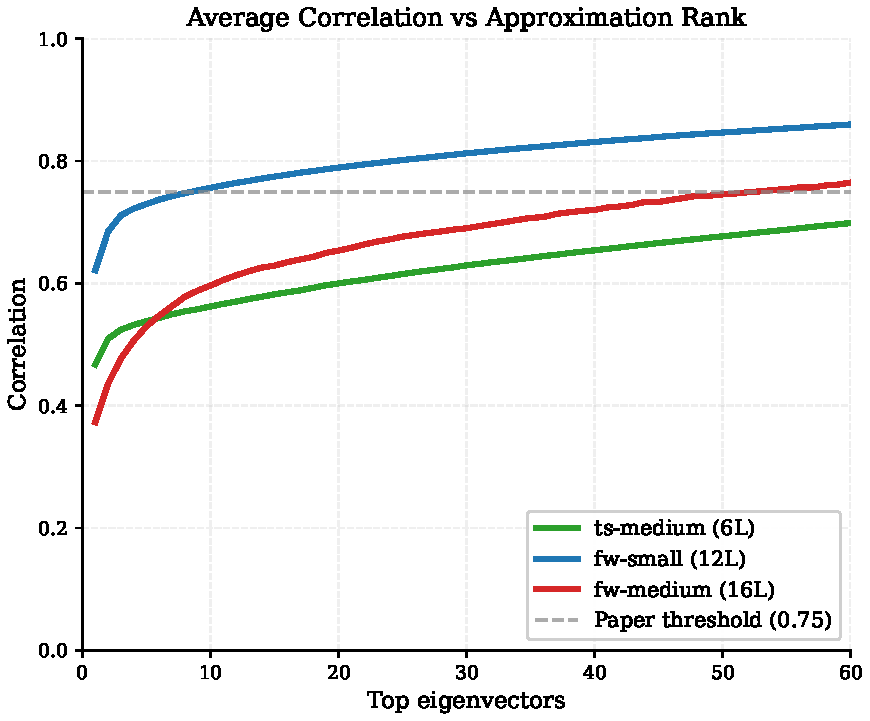
\includegraphics[width=\textwidth,height=0.32\textheight,keepaspectratio]{../Report/figures/language/figure_9a_correlation_progression.pdf}
        {\tiny Correlation vs rank $k$}
        
        \column{0.4\textwidth}
        \centering
        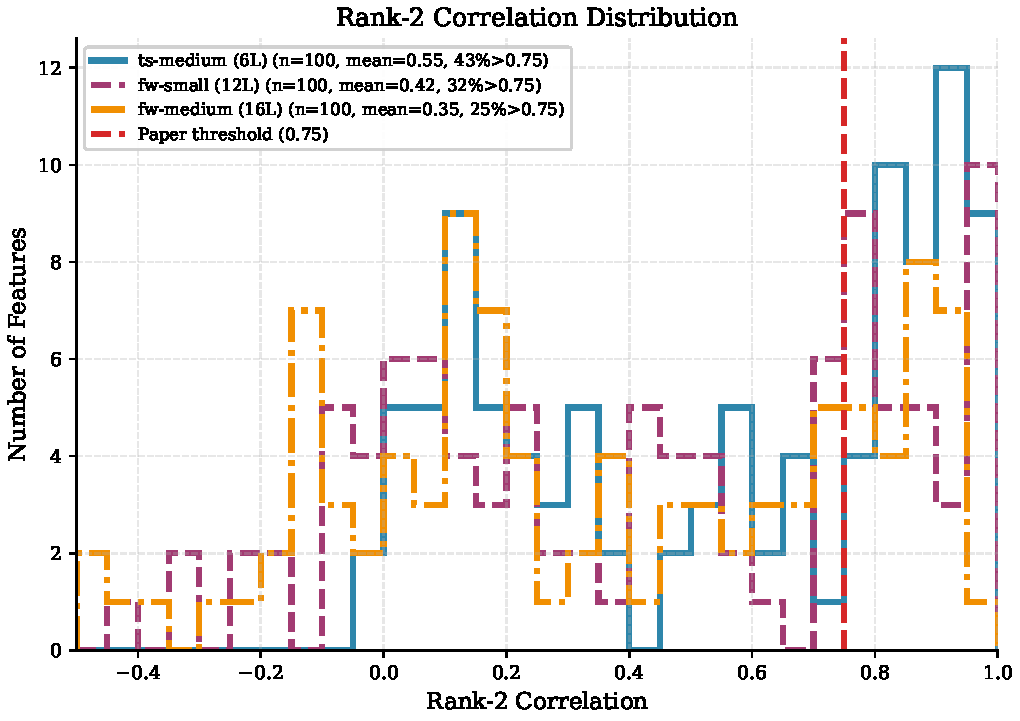
\includegraphics[width=\textwidth,height=0.32\textheight,keepaspectratio]{../Report/figures/language/figure_9b_correlation_histogram.pdf}
        {\tiny Rank-2 correlation histogram}
        
        \column{0.2\textwidth}
        \scriptsize
        \textbf{Why vary?}\\
        Higher tok/param $\to$ better low-rank behavior
        
        \vspace{0.1cm}
        \fcolorbox{black}{yellow!20}{
            \parbox{0.9\textwidth}{\tiny
                L3 $\sim$ \quad L5 $\sim$\\
                (partial)
            }
        }
    \end{columns}
\end{frame}

\begin{frame}{Language: Training Time Effect (Figure 10)}
    \begin{columns}[T]
        \column{0.55\textwidth}
        \centering
        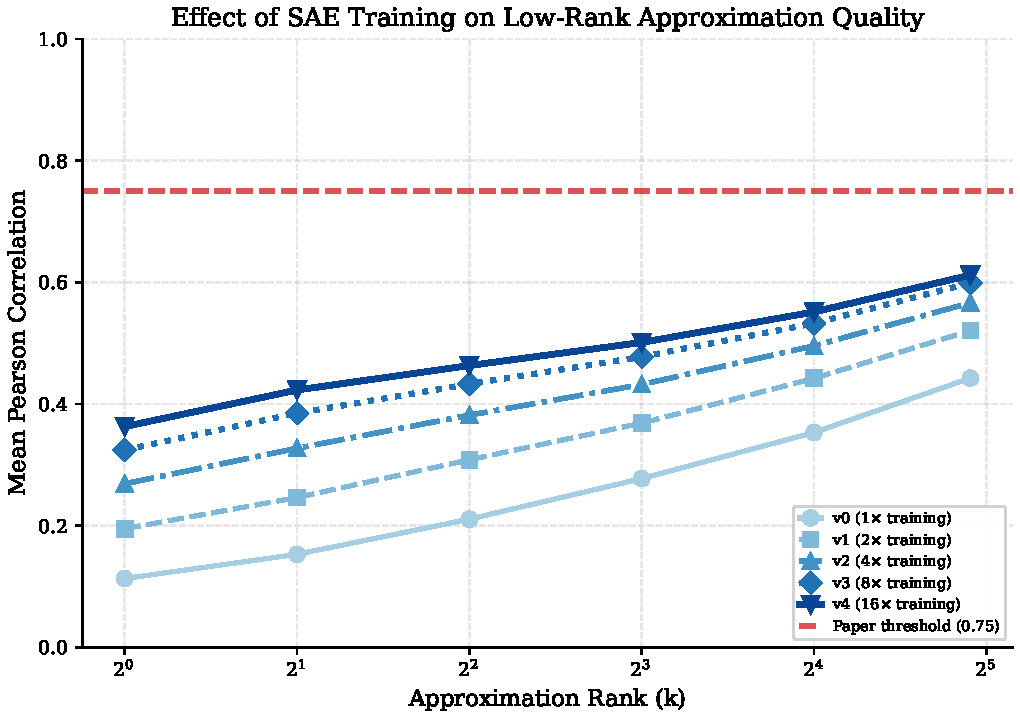
\includegraphics[width=\textwidth,height=0.55\textheight,keepaspectratio]{../Report/figures/language/figure_10a_sae_training_effect.pdf}
        
        \column{0.45\textwidth}
        \small
        \textbf{Hypothesis:} Low-rank emergence requires sufficient training.
        
        \vspace{0.2cm}
        \textbf{Evidence:} SAE training progression (v0 $\to$ v4) shows:
        \begin{itemize}
            \item Fraction of features with corr $>$ 0.75 increases \textbf{2.5$\times$}
            \item More training $\to$ better low-rank structure
        \end{itemize}
        
        \vspace{0.2cm}
        \textbf{Tokens/param ratio:}
        \begin{itemize}
            \item fw-small: 198 $\to$ 65\% high corr
            \item fw-medium: 99 $\to$ 45\%
            \item ts-medium: 83 $\to$ 32\%
        \end{itemize}
        
        \vspace{0.1cm}
        \scriptsize
        Models trained longer (higher tok/param) show stronger low-rank behavior.
    \end{columns}
\end{frame}

\begin{frame}{Reproduction Summary}
    \begin{table}[h]
        \centering
        \footnotesize
        \begin{tabular}{lp{3.5cm}cp{4cm}}
            \toprule
            ID & Description & Status & Notes \\
            \midrule
            \multicolumn{4}{c}{\textit{Vision (Section 4)}} \\
            \midrule
            V1 & Low-rank emergence & \checkmark & EffRank: 15.5 vs.\ 38.5 \\
            V2 & Interpretable eigenvectors & \checkmark & Clear digit patterns \\
            V3 & Overfitting without reg. & \checkmark & Diffuse patterns \\
            V4 & Regularization roles & \checkmark & WD $\downarrow$ rank; noise $\uparrow$ acc \\
            V5 & Cross-seed consistency & \checkmark & Top eigenvecs similar; acc low std \\
            V6 & Adversarial generation & \checkmark & Eigenvector attacks work \\
            \midrule
            \multicolumn{4}{c}{\textit{Language (Section 5)}} \\
            \midrule
            L1 & SAE feature discovery & \checkmark & Pretrained SAEs work \\
            L2 & Negation circuits & \checkmark & AND-gate confirmed \\
            L3 & Low-rank interactions & $\sim$ & 32--65\% $>$0.75 \\
            L4 & Sparse interactions & \checkmark & Block structure found \\
            L5 & Cross-model generalization & $\sim$ & Method works; varies \\
            \bottomrule
        \end{tabular}
    \end{table}
\end{frame}
